%%% File-Information {{{
%%% Filename: template_bericht.tex
%%% Purpose: lab report, technical report, project report
%%% Time-stamp: <2004-06-22 23:36:32 xx>
%%% Authors: The LaTeX@TUG-Team [http://latex.tugraz.at/]:
%%%          Karl Voit (vk), Michael Prokop (mp), Stefan Sollerer (ss)
%%% History:
%%%   20040625 (vk,ss) initial version
%%%
%%% Notes:
%%%
%%%
%%%
%%% }}}
%%%%%%%%%%%%%%%%%%%%%%%%%%%%%%%%%%%%%%%%%%%%%%%%%%%%%%%%%%%%%%%%%%%%%%%%%%%%%%%%
%%% main document {{{

\documentclass[
a4paper,     %% defines the paper size: a4paper (default), a5paper, letterpaper, ...
% landscape,   %% sets the orientation to landscape
% twoside,     %% changes to a two-page-layout (alternatively: oneside)
% twocolumn,   %% changes to a two-column-layout
 headsepline, %% add a horizontal line below the column title
% footsepline, %% add a horizontal line above the page footer
% titlepage,   %% only the titlepage (using titlepage-environment) appears on the first page (alternatively: notitlepage)
 parskip=half,
% halfparskip,     %% insert an empty line between two paragraphs (alternatively: halfparskip, ...)
% leqno,       %% equation numbers left (instead of right)
 fleqn,       %% equation left-justified (instead of centered)
% tablecaptionabove, %% captions of tables are above the tables (alternatively: tablecaptionbelow)
% draft,       %% produce only a draft version (mark lines that need manual edition and don't show graphics)
% 10pt         %% set default font size to 10 point
% 11pt         %% set default font size to 11 point
12pt         %% set default font size to 12 point
]{scrartcl}  %% article, see KOMA documentation (scrguide.dvi)



%%%%%%%%%%%%%%%%%%%%%%%%%%%%%%%%%%%%%%%%%%%%%%%%%%%%%%%%%%%%%%%%%%%%%%%%%%%%%%%%
%%%
%%% packages
%%%

%%%
%%% encoding and language set
%%%
\usepackage[utf8]{inputenc}
\usepackage[T1]{fontenc}
\usepackage{ngerman} % which should have the same result as \usepackage[ngerman]{babel}
\usepackage{float}

%%%
%%% technical packages
%%%

%%% amsmath, amssymb, amstext: support for mathematics
\usepackage{amsmath,amssymb,amstext}

%%% psfrag: replace PostScript fonts
%\usepackage{psfrag}


%%% units: technical units
\usepackage{units}

%% listings: sourcecode
\usepackage{listings}

%% colors
\usepackage{color}

\definecolor{mygreen}{rgb}{0,0.6,0}
\definecolor{mygray}{rgb}{0.5,0.5,0.5}
\definecolor{mymauve}{rgb}{0.58,0,0.82}

%%%
%%% layout
%%%

%%% scrpage2: KOMA heading and footer
%%% Note: if you don't use this package, please remove 
%%%       \pagestyle{scrheadings} and corresponding settings
%%%       below too.
\usepackage{scrpage2}

%%%
%%% PDF
%%%

%%%\newif\ifpdf
%%%  \ifx\pdfoutput\undefined
%%%     \pdffalse
%%%  \else
%%%     \pdfoutput=1
%%%     \pdftrue
%%%  \fi

%%% Should be LAST usepackage-call!
%%% For docu on that, see reference on package ``hyperref''
\ifpdfoutput{%   (definitions for using pdflatex instead of latex)

  %%% graphicx: support for graphics
  \usepackage[pdftex]{graphicx}

  \pdfcompresslevel=9

  %%% hyperref (hyperlinks in PDF): for more options or more detailed
  %%%          explanations, see the documentation of the hyperref-package
  \usepackage[%
    %%% general options
    pdftex=true,      %% sets up hyperref for use with the pdftex program
    %plainpages=false, %% set it to false, if pdflatex complains: ``destination with same identifier already exists''
    %
    %%% extension options
    backref=true,      %% if true, adds a backlink text to the end of each item in the bibliography
    pagebackref=false, %% if true, creates backward references as a list of page numbers in the bibliography
    colorlinks=false,   %% turn on colored links (true is better for on-screen reading, false is better for printout versions)
    %
    %%% PDF-specific display options
    bookmarks=true,          %% if true, generate PDF bookmarks (requires two passes of pdflatex)
    bookmarksopen=false,     %% if true, show all PDF bookmarks expanded
    bookmarksnumbered=false, %% if true, add the section numbers to the bookmarks
    %pdfstartpage={1},        %% determines, on which page the PDF file is opened
    pdfpagemode=None         %% None, UseOutlines (=show bookmarks), UseThumbs (show thumbnails), FullScreen
  ]{hyperref}


  %%% provide all graphics (also) in this format, so you don't have
  %%% to add the file extensions to the \includegraphics-command
  %%% and/or you don't have to distinguish between generating
  %%% dvi/ps (through latex) and pdf (through pdflatex)
}{%else   (definitions for using latex instead of pdflatex)
  \usepackage[dvips]{graphicx}

  \usepackage[%
    dvips,           %% sets up hyperref for use with the dvips driver
    colorlinks=false %% better for printout version; almost every hyperref-extension is eliminated by using dvips
  ]{hyperref}

}


%%% sets the PDF-Informations options
%%% (see fields in Acrobat Reader: ``File -> Document properties -> Summary'')
%%% Note: this method is better than as options of the hyperref-package (options are expanded correctly)
\hypersetup{
  pdftitle={Untersuchung einer Antriebswelle}, %%
  pdfauthor={Schmid}, %%
  pdfsubject={}, %%
  pdfcreator={Accomplished with LaTeX2e and pdfLaTeX with hyperref-package.}, %% 
  pdfproducer={}, %%
  pdfkeywords={} %%
}


%%%%%%%%%%%%%%%%%%%%%%%%%%%%%%%%%%%%%%%%%%%%%%%%%%%%%%%%%%%%%%%%%%%%%%%%%%%%%%%%
%%%
%%% user defined commands
%%%

%%% \mygraphics{}{}{}
%% usage:   \mygraphics{width}{filename_without_extension}{caption}
%% example: \mygraphics{0.7\textwidth}{rolling_grandma}{This is my grandmother on inlinescates}
%% requires: package graphicx
%% provides: including centered pictures/graphics with a boldfaced caption below
%% 
\newcommand{\mygraphics}[3]{
  \begin{center}
    \includegraphics[width=#1, keepaspectratio=true]{#2} \\
    \textbf{#3}
  \end{center}
}

%%%%%%%%%%%%%%%%%%%%%%%%%%%%%%%%%%%%%%%%%%%%%%%%%%%%%%%%%%%%%%%%%%%%%%%%%%%%%%%%
%%%
%%% define the titlepage
%%%

 \subject{Semesterarbeit}   %% subject which appears above titlehead
% \titlehead{} %% special heading for the titlepage

%%% title
\title{Evaluation von verschiedenen Ansätzen für Evolutionäre Algorithmen}

%%% author(s)
\author{Adrian Schmid}

%%% date
\date{Zürich, 01.01.2014}

% \publishers{}

% \thanks{} %% use it instead of footnotes (only on titlepage)

% \dedication{} %% generates a dedication-page after titlepage


%%% uncomment following lines, if you want to:
%%% reuse the maketitle-entries for hyperref-setup
%\newcommand\org@maketitle{}
%\let\org@maketitle\maketitle
%\def\maketitle{%
%  \hypersetup{
%    pdftitle={\@title},
%    pdfauthor={\@author}
%    pdfsubject={\@subject}
%  }%
%  \org@maketitle
%}


%%%%%%%%%%%%%%%%%%%%%%%%%%%%%%%%%%%%%%%%%%%%%%%%%%%%%%%%%%%%%%%%%%%%%%%%%%%%%%%%
%%%
%%% set heading and footer
%%%

%%% scrheadings default: 
%%%      footer - middle: page number
\pagestyle{scrheadings}

%%% user specific
%%% usage:
%%% \position[heading/footer for the titlepage]{heading/footer for the rest of the document}

%%% heading - left
% \ihead[]{}

%%% heading - center
% \chead[]{}

%%% heading - right
 \ohead[]{Evaluation von verschiedenen Ansätzen für Evolutionäre Algorithmen}

%%% footer - left
% \ifoot[]{}

%%% footer - center
% \cfoot[]{}

%%% footer - right
% \ofoot[]{}



%%%%%%%%%%%%%%%%%%%%%%%%%%%%%%%%%%%%%%%%%%%%%%%%%%%%%%%%%%%%%%%%%%%%%%%%%%%%%%%%
%%%
%%% begin document
%%%

\setcounter{tocdepth}{2}


\begin{document}

  \lstset{ %
    backgroundcolor=\color{white},   % choose the background color; you must add \usepackage{color} or \usepackage{xcolor}
    basicstyle=\footnotesize,        % the size of the fonts that are used for the code
    breakatwhitespace=false,         % sets if automatic breaks should only happen at whitespace
    breaklines=true,                 % sets automatic line breaking
    captionpos=b,                    % sets the caption-position to bottom
    commentstyle=\color{mygreen},    % comment style
    deletekeywords={...},            % if you want to delete keywords from the given language
    escapeinside={\%*}{*)},          % if you want to add LaTeX within your code
    extendedchars=true,              % lets you use non-ASCII characters; for 8-bits encodings only, does not work with UTF-8
    frame=single,                    % adds a frame around the code
    keepspaces=true,                 % keeps spaces in text, useful for keeping indentation of code (possibly needs columns=flexible)
    keywordstyle=\color{blue},       % keyword style
    language=Octave,                 % the language of the code
    morekeywords={*,...},            % if you want to add more keywords to the set
    numbers=left,                    % where to put the line-numbers; possible values are (none, left, right)
    numbersep=5pt,                   % how far the line-numbers are from the code
    numberstyle=\tiny\color{mygray}, % the style that is used for the line-numbers
    rulecolor=\color{black},         % if not set, the frame-color may be changed on line-breaks within not-black text (e.g. comments (green here))
    showspaces=false,                % show spaces everywhere adding particular underscores; it overrides 'showstringspaces'
    showstringspaces=false,          % underline spaces within strings only
    showtabs=false,                  % show tabs within strings adding particular underscores
    stepnumber=1,                    % the step between two line-numbers. If it's 1, each line will be numbered
    stringstyle=\color{mymauve},     % string literal style
    tabsize=2,                       % sets default tabsize to 2 spaces
  }



 \pagenumbering{roman} %% small roman page numbers

%%% include the title
% \thispagestyle{empty}  %% no header/footer (only) on this page
 \maketitle

\clearpage
\section*{Dank}
Ich danke Bla und Bli

\clearpage
\topskip0pt
\vspace*{\fill}
\section*{\centering Zusammenfassung}
Diese Semesterarbeit beschäftigt sich mit Grundlagen der Automatentheorie, Grundlagen von evolutionären Algorithmen und schliesslich einem konkreten praktischen Anwendungsfall dieser theoretischen Gebiete. Es geht um das finden von endlichen Automaten zu gegebenen regulären Ausdrücken mithilfe von evolutionären Algorithmen. Dabei wird das Verhalten von Algorithmen mit unterschiedlichen relativen Fitnessfunktionen betrachtet. Die Qualität der Resultate und der dazu benötigte Rechenaufwand wird verglichen um so die Stärken und Schwächen der verschiedenen Herangehensweisen zu aufzuzeigen.
\vspace*{\fill}




\clearpage
%%% start a new page and display the table of contents
% \newpage
 \tableofcontents


%%% display the main document on a new page 
% \newpage

 \pagenumbering{arabic} %% normal page numbers (include it, if roman was used above)

%%%%%%%%%%%%%%%%%%%%%%%%%%%%%%%%%%%%%%%%%%%%%%%%%%%%%%%%%%%%%%%%%%%%%%%%%%%%%%%%
%%%
%%% begin main document
%%% structure: \section \subsection \subsubsection \paragraph \subparagraph
%%%

\clearpage
\section{Einleitung}
\subsection{Ausgangslage}
Evolutionäre Algorithmen sind Optimierungsverfahren die sich, inspiriert durch in der Natur ablaufende Prozesse, den grundlegenden evolutionären Mechanismen von Mutation, Selektion und Rekombination bedienen. In dieser Arbeit werden verschiedene Selektionsstrategien an einem einfachen Beispiel miteinander verglichen.

\subsection{Ziel der Arbeit}
Ziel der Arbeit ist es, an einem einfachen Beispiel, verschiedene Ansätze zum Entwurf von relativen Fitnessfunktionen gegeneinander abzuwägen. Dazu werden evolutionäre Algorithmen mit unterschiedlichen Strategien implementiert. Die aus den unterschiedlichen Ansätzen resultierenden Lösungen werden dann hinsichtlich ihrer Qualität und der für ihre Suche benötigten Ressourcen (Rechenzeit) verglichen.

\subsection{Aufgabenstellung}
In dieser Arbeit sollen evolutionäre Algorithmen implementiert welchen, welche zu einem gegebenen Regulären Ausdruck einen entsprechenden endlichen Automaten finden. Für dieses konkrete Beispiel sollen evolutionäre Algorithmen mit verschiedenen Strategien implementiert werden, umso das Konvergenzverhalten und die Rechenzeit der verschiedenen Implementationen (und somit der Strategien) untersuchen und vergleichen zu können.
\begin{itemize}
	\item Einarbeitung in das Thema
	\item Repräsentation und Mutation von endlichen Automaten definieren 
	\item Evolutionärer Algorithmus mit fester, globaler Problemmenge implementieren 
	\item Evolutionärer Algorithmus mit mutierender, globaler Problemmenge implementieren 
	\item Evolutionärer Algorithmus, bei welchem jeder Lösungskandidat seine eigene, mutierende Problemmenge mitführt implementieren
	\item Gegenüberstellung der Resultate
\end{itemize}

\subsection{Erwartete Resultate}
\begin{itemize}
	\item Überblick über Evolutionäre Algorithmen und Endliche Automaten im technischen Bericht
	\item Implementierung einer Repräsentation von endlichen Automaten, Implementierung von Mutationen zu endlichen Automaten und Dokumentation des Implementierten im technischen Bericht 
	\item Implementierung eines evolutionären Algorithmus mit fester, globaler Problemmenge mit einer entsprechenden Dokumentation im technischen Bericht 
	\item Implementierung eines evolutionären Algorithmus mit mutierender, globaler Problemmenge mit einer entsprechenden Dokumentation im technischen Bericht 
	\item Implementierung eines evolutionären Algorithmus, bei welchem jeder Lösungskandidat seine eigene, mutierende Problemmenge mitführt mit einer entsprechenden Dokumentation im technischen Bericht 
	\item Dokumentation der Gegenüberstellung der Resultate
\end{itemize}

\clearpage
\section{Grundlagen}
\subsection{Endliche Automaten und reguläre Sprachen}
Reguläre Sprachen und endliche Automaten gehören zur Automatentheorie, einem Teilbereich der theoretischen Informatik. Zum besseren Verständnis dieser Arbeit wurden folgend einige gängige und wichtige Konzepte der Automatentheorie frei nach dem Standartwerk von Hopcroft, Motwani und Ullman zusammengefasst. \cite{hopcroft}
 
\paragraph{Alphabet}
Ein Alphabet ist eine endliche, nicht leere Menge von Symbolen. Üblicherweise wird ein Alphabet durch das Symbol $\Sigma$ dargestellt.
\paragraph{Zeichenreihen}
Eine Zeichenreihe (auch Wort oder String) ist eine endliche Folge von Symbolen eines bestimmten Alphabetes.
\paragraph{Sprachen}
Eine Menge von Zeichenreihen aus $\Sigma^*$, wobei $\Sigma$ ein bestimmtes Alphabet darstellt, wird als Sprache bezeichnet. Das heisst, eine Sprache ist eine Menge von Zeichenreihen die mit den Zeichen aus einem Alphabet $\Sigma$ gebildet werden können. Bei der Bildung von Wörtern müssen nicht alle Zeichen des gegebenen Alphabets verwendet werden.

Bei der Klasse der regulären Sprachen handelt es sich um die Menge aller Sprachen, welche durch einen endlichen Automaten beschrieben werden können. Alle Sprachen dieser Klasse können auch durch einen regulären Ausdruck dargestellt werden. Das heisst, dass es für jede reguläre Sprache sowohl einen regulären Ausdruck als auch einen endlichen Automaten gibt, der alle Wörter der Sprache akzeptiert.

Ein deterministischer endlicher Automat besteht gemäss Hopcroft, Motwani und Ullman \cite{hopcroft} aus:
\begin{enumerate}
  \item einer endlichen menge von Zuständen die meist durch $Q$ bezeichnet wird.
  \item einer endlichen Menge von Eingabesymbolen (auch Alphabet $\Sigma$).
  \item einer Übergangsfunktion $\delta$ der ein Zustand und ein Eingabesymbol übergeben werden und die einen Zustand zurückgibt.
  \item einem Startzustand welcher Teil der Menge $Q$ sein muss.
  \item einer Menge $F$ akzeptierender Zustände. Die Menge $F$ ist eine Teilmenge von $Q$.
\end{enumerate}

Oft werden endliche Automaten als Quintupel in der Form $A$ = ($Q$, $\Sigma$, $\delta$, $q0$, $F$) dargestellt. 

Zum besseren Verständnis folgend ein Beispiel eines Automaten welcher alle Binärzahlen die durch drei teilbar sind akzeptiert.
\begin{figure}[h]
  \centering
  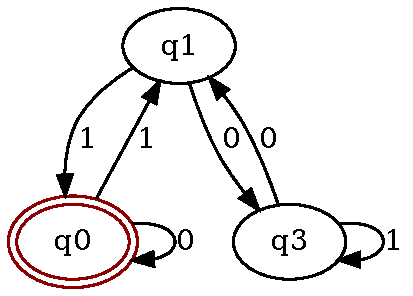
\includegraphics{images/endlicher_automat.pdf}
  \caption[Beispiel: Endlicher Automat]{Beispiel: Endlicher Automat}
  \label{fig:endlicher_automat}
\end{figure}

Die Attribute des Quintupels für diesen Automaten sind:
\begin{enumerate}
	\item $Q$ = \{$q0$, $q1$, $q3$\}
	\item $\Sigma$ = \{$0$, $1$\}
	\item $\delta$
	\item $q0$
	\item $F$ = \{$q0$\}
\end{enumerate}
Wobei man die Übergangsfunktion $\delta$ am einfachsten als Tabelle wie folgt darstellt:
\begin{table}[h]
	\centering
	\begin{tabular}{ c || c | c }
	  \hline
	   & 0 & 1 \\
	  \hline  
	  $\rightarrow$q0* & q0 & q1 \\
	  q1 & q3 & q0 \\
	  q3 & q1 & q3 \\
	  \hline  
	\end{tabular}
	\caption[Übergangstabelle]{Übergangstabelle}
\end{table}

\paragraph{Konventionen}
Ich habe mich bei der Darstellung von Automaten im Rahmen dieser Arbeit auf folgende Konvention festgelegt:
\begin{itemize}
	\item Zustände werden mit einem kleinen q gefolgt von einer Zahl bezeichnet (zB. $q1$)
	\item Zustände müssen nicht durchgängig nummeriert sein
	\item Zustände werden als Ellipsen dargestellt
	\item Zustandsübergänge sind beschriftete Pfeile
	\item der Startzustand erhält einen roten Rand
	\item alle akzeptierenden Zustände sind doppelt umrandet
\end{itemize}
\subsection{Evolutionäre Algorithmen}
'Unter evolutionären Algorithmen (EA) verstehen wir randomisierte Heuristiken, die Suchprobleme näherungsweise durch vereinfachende algorithmische Umsetzung von
Prinzipien der natürlichen Evolution zu lösen versuchen. Somit geben evolutionäre Algorithmen in der Regel weder eine Garantie bzgl. der benätigten Rechenzeit noch der Güte der ausgegebenen Lösung. Ein Suchproblem besteht darin, zu einer Zielfunktion ein Element aus deren Definitionsbereich zu finden, dessen Funktionswert möglichst gut ist. Darunter verstehen wir im Folgenden, wenn nicht ausdrücklich anders vermerkt, einen möglichst grossen Funktionswert, weshalb der Zielfunktions wert eines Elements auch als seine Fitness bezeichnet wird.

Der Aufbau eines evolutionären Algorithmus lässt sich dann grob wie folgt beschreiben: in jedem Schritt verwaltet er eine Menge fester Grösse von Suchpunkten, die so genannte Population, wobei jeder einzelne Suchpunkt auch als Individuum bezeichnet wird. Aus den Punkten der Population neue Punkte zu erzeugen, ist Aufgabe von Mutation und Rekombination. Dabei steht hinter der Mutation die Idee, jeweils nur ein einzelnes Individuum zufällig zu verändern, ohne dass andere Individuen dabei berücksichtigt werden. Durch Rekombination wird hingegen aus mehreren, meist zwei Individuen zufällig ein neues gebildet, das von diesen möglichst gute Eigenschaften übernehmen soll. Durch Mutation und Rekombination werden also neue Individuen (Kinder genannt) aus bestehenden Individuen (Eltern genannt) erzeugt. Beide Operatoren hängen oftmals stark von Zufallsentscheidungen ab. Jedoch fliesst in der Regel weder in Mutation noch Rekombination der Zielfunktionswert der Individuen ein.

Die Zielfunktion beeinflusst nur die Selektion. Dieser Operator wählt Individuen der Population aus, sei es zur Auswahl der Eltern für eine Rekombination oder Mutation oder, um aus der Menge von Eltern und Kindern die nächste Population zu wählen, was den Übergang zur nächsten Generation darstellt. Dadurch, dass die Selektion Punkte mit höherem Zielfunktionswert mit grösserer Wahrscheinlichkeit auswählt, soll erreicht werden, dass nach und nach immer bessere Punkte gefunden werden.' \cite{droste}

\begin{figure}[h]
  \centering
  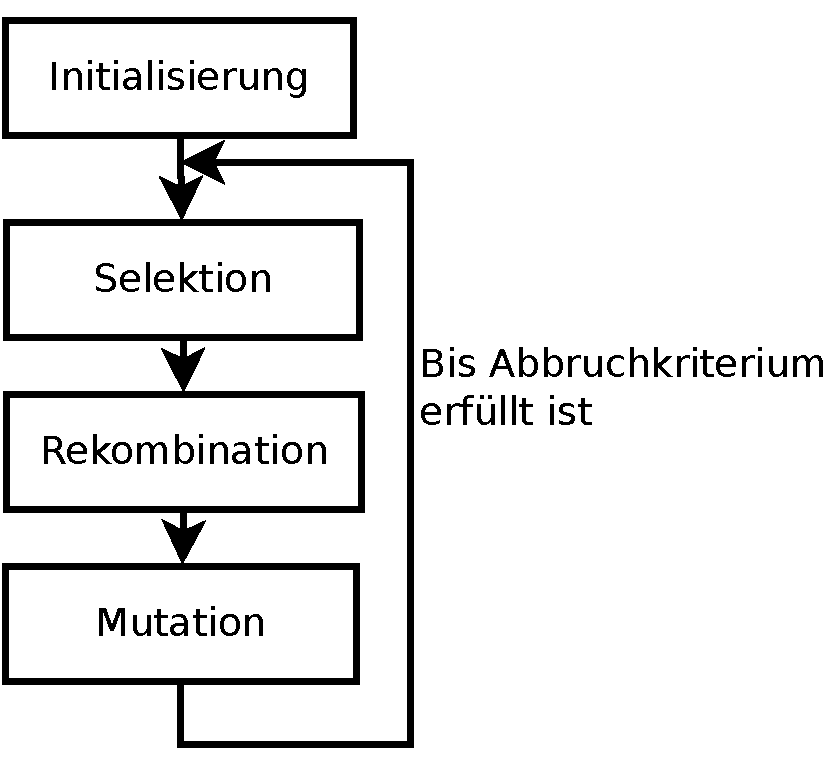
\includegraphics[width=0.5\textwidth]{images/evolutionaerer_algorithmus.pdf}
  \caption[Evolutionärer Algorithmus]{Evolutionärer Algorithmus}
  \label{fig:endlicher_automat}
\end{figure}

\subsubsection{Anwendung auf unser Problem}
Unser Problem der Findung von regulären Automaten welche die selbe Sprache akzeptieren wie ein gegebener regulärer Ausdruck läst sich wie mit einigen Anpassungen in diesem Standartmodell eines evolutionären Algorithmus abbilden.

\paragraph{Initialisierung}
In der Initialisierungsphase werden wir eine Population von Automaten zufällig erzeugen. Das heisst wir erzeugen eine Zufällige Anzahl von Zuständen, verbinden diese Zufällig und setzen einen zufälligen Start und zufällige Akzeptierende Zustände.

\paragraph{Selektion}
Es werden jeweils diejenigen Automaten selektiert welche eine höhere Fitness aufweisen. Es werden verschiedene Ansätze zur Selektion implementiert und es wird deren Konvergenzverhalten analysiert.

\paragraph{Fitness}
Die Fitness von Automaten bestimmen wir in dem wir ihn mit Wörtern füttern und die Ausgabe mit der soll Ausgabe vergleichen. Die Soll Ausgabe können wir anhand des gegebenen regulären Ausdrucks einfach bestimmen. Der Wert der Fitnessfunktion entspricht dann der Summe der richtig akzeptierten und richtig nicht akzeptierten Wörtern aus unserer \textit{Problemmenge}.

\paragraph{Problemmenge}
Die Problemmenge ist eine Menge von Tupeln ($Wort$, $Soll Ausgabe$) welche verwendet wird um die Fitness von Automaten zu bestimmen. Im Rahmen dieser Arbeit werden unter anderem Verschiedene Ansätze zur Erzeugung und zum Verhalten solcher Problemmengen ausprobiert. Dabei wird das Konvergenzverhalten des evolutionären Algorithmus untersucht.

\paragraph{Rekombination}
Wenn man zwei endliche Automaten graphisch zusammenfügt, wird der resultierende Automat ein komplett anderes Verhalten aufweisen als die beiden Eltern. Deshalb verzichten wir auf die rekombination im herkömmlichen Sinne. Wir klonen jeweils die selektierten Automaten und \textit{mutieren} die so entstandenen Kinder.

\paragraph{Mutation}
Bei der Mutation soll jeweils eine zufällige Veränderung an einem Automaten durchgeführt werden. Wir haben uns auf folgende Mutationen festgelegt:
\begin{enumerate}
	\item einen Zustand hinzufügen
	\item einen Zustand entfernen
	\item eine Verbindung zwischen zwei Zuständen ändern
	\item einen nicht akzeptierenden Zustand zu einem akzeptierenden Zustand umwandeln
	\item einen akzeptierenden Zustand zu einem nicht akzeptierenden Zustand umwandeln
\end{enumerate}
\clearpage
\section{Umsetzung}
\subsection{Automaten}

\begin{figure}[h]
  \centering
  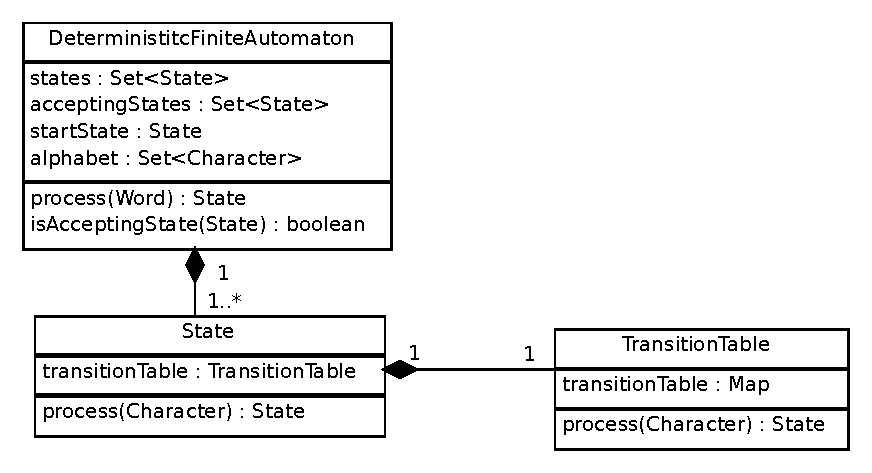
\includegraphics[width=0.5\textwidth]{images/dfa_classdiag_simple.pdf}
  \caption[DFA Klassendiagramm vereinfacht]{DFA Klassendiagramm vereinfacht}
  \label{fig:dfa_classdiag_simple}
\end{figure}


Das Quintupel Modell ($Q$, $\Sigma$, $\delta$, $q0$, $F$) wurde wie folgt implementiert:

\begin{tabular}{ l | l }
  \hline
  $Q$ & Die Menge der Zustände wurde als Set von States implementiert.  \\
  \hline
  $\Sigma$ & 5 \\
  \hline
  $\delta$ & 8 \\
  \hline
  $\q0$ & 8 \\
  \hline
  $F$ & 8 \\
  \hline 
\end{tabular}


\subsection{Evolutionäre Algorithmen}
Bei der Implementierung der Evolutionären Ansätze wurde insbesondere Wert darauf gelegt, dass sowohl die theoretischen Grundlagen abgebildet sind als auch dass die verschiedenen Ansätze mit der grundsätzlich selben Struktur implementiert werden können um Redundanz im Code so gut als möglich zu vermeiden. Mit diesen Zielen vor Augen wurde folgende Grundstruktur für die Implementierung von evolutionären Algorithmen entworfen:

\begin{figure}[h]
  \centering
  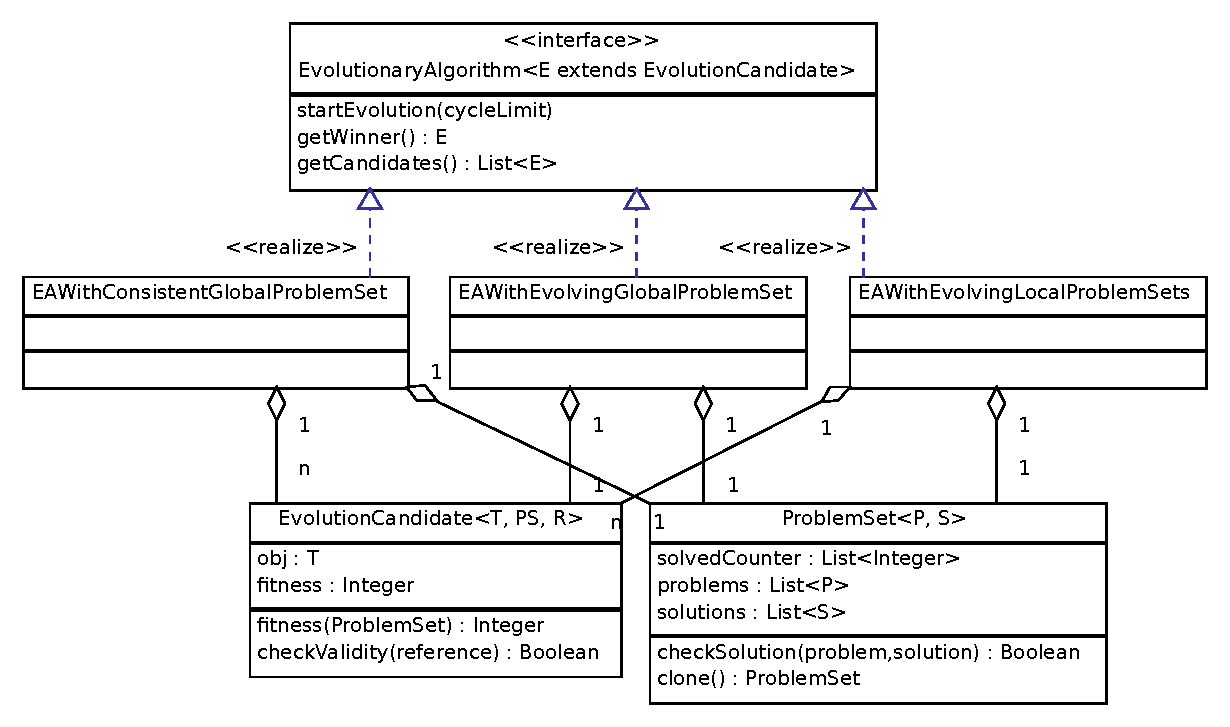
\includegraphics[width=0.8\textwidth]{images/simple_uml_evolution.pdf}
  \caption[EA Grundstruktur Klassendiagramm]{EA Grundstruktur vereinfacht}
  \label{fig:ea_classdiag_simple}
\end{figure}

Die Klassen welche die Algorithmen beinhalten verwenden eine Menge von \lstinline$EvolutionCandidate$ (Population) und ein \lstinline$ProblemSet$. Der evolutionäre Algorithmus kann jeweils mit \lstinline$startEvolution$ gestartet werden und wird abgebrochen sobald eine gültige Lösung gefunden wurde.

Das \lstinline$ProblemSet$ besteht Grundsätzlich aus zwei Listen. In der Ersten ist die \flqq Problemstellung\frqq abgelegt, in der zweiten die entsprechenden Musterlösung. Mithilfe der Methode \lstinline$checkSolution(problem, solution)$ kann geprüft werden ob eine erarbeite Lösung (Parameter \lstinline$solution$) der Musterlösung entspricht. In unserem Fall wird so geprüft, ob unser Automat die Zugehörigkeit eines Wortes zu der gegebenen Sprache richtig erkennt oder nicht.

Der \lstinline$EvolutionCandidate$ entspricht einem Individuum aus unserer Population und besteht aus dem \flqq obj\frqq, welches in unserem Fall den Automaten an sich beinhaltet, der \lstinline$fitness$ als Eigenschaft (wird zur Sortierung verwendet) und einer \lstinline$fitness$ Funktion welche ein \lstinline$ProblemSet$ entgegen nimmt und mithilfe des gegebenen \flqq obj\frqq versucht alle Probleme aus dem \lstinline$ProblemSet$ zu lösen. Die Fitness als Wert entspricht der Anzahl korrekt gelöster Probleme.

\subsubsection{Initialisierung}
Um die Klassen der evolutionären Algorithmen schlank zu halten, wurde die Initialisierung ausgelagert. In der Abbildung \ref{fig:ea_init_classdiag_simple} sieht man, dass die Initialisierung eines evolutionären Algorithmus zur Findung eines endlichen Automaten zu einem gegebenen regulären Ausdruck in drei Schritten abläuft:
\begin{enumerate}
	\item Sprache initialisieren (\lstinline$initLanguage(alphabet, maxWordLength, regexp)$)
	\item Probleme initialisieren (\lstinline$initProblems(noProblems)$)
	\item Population initialisieren (\lstinline$initCandidates(noCandidates)$)
\end{enumerate}

\begin{figure}[h]
  \centering
  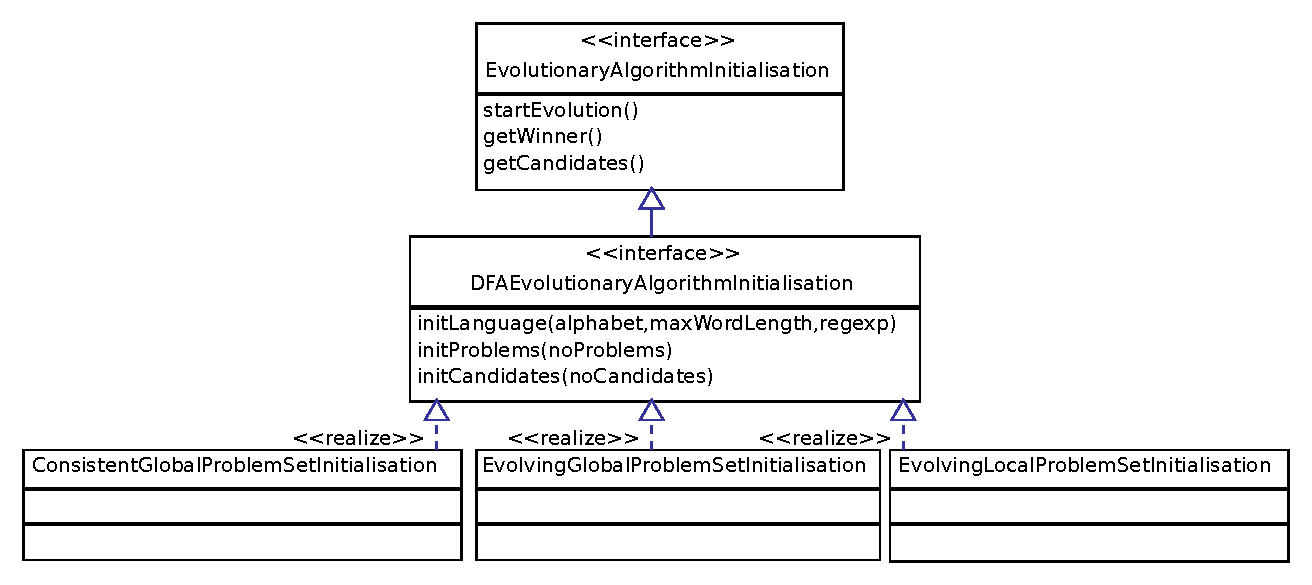
\includegraphics[width=0.8\textwidth]{images/simple_uml_evolution_initialisation.pdf}
  \caption[EA Initialisierung Klassendiagramm]{EA Initialisierung Klassendiagramm}
  \label{fig:ea_init_classdiag_simple}
\end{figure}

\paragraph{Initialisierung der Sprache}
Beim initialisieren der Sprache werden das Alphabet und der reguläre Ausdruck für die spätere Verwendung abgelegt, es wird eine Instanz des \lstinline$WordProblemGenerator$s angelegt und ein Referenzautomat (\lstinline$dk.brics.automaton$) wird erzeugt, welcher später zur Überprüfung von Resultaten verwendet wird.

\paragraph{Generieren von Problemen}
Probleme werden von einem \lstinline$ProblemGenerator$ erzeugt. Die für dieses Problem erstellte Implementation \lstinline$WordProblemGenerator$ generiert mithilfe eines gegebenen Alphabets Tupel vom Typ \lstinline$Tuple<CharArray, Boolean>$ wobei im \lstinline$CharArray$ eine zufällige Zeichenfolge der Zeichen aus dem Alphabet mit einer zufälligen länge zwischen 0 und \lstinline$maxWordLength$ Zeichen ist. Der Boolean zeigt an, ob die generierte Zeichenfolge vom ebenfalls gegebenen \lstinline$regexp$ akzeptiert wird oder nicht.

Zu dem generieren von einzelnen \flqq Problem\frqq - \flqq Lösung\frqq Tupeln kann der Problemgenerator auch ganze ProblemSets generieren. Als Parameter hierfür benötigt der \lstinline$WordProblemGenerator$ die gewünschte Länge des Sets und ein Flag welches angibt ob der leere String immer im Set vorhanden sein soll oder nicht.

\begin{figure}[h]
  \centering
  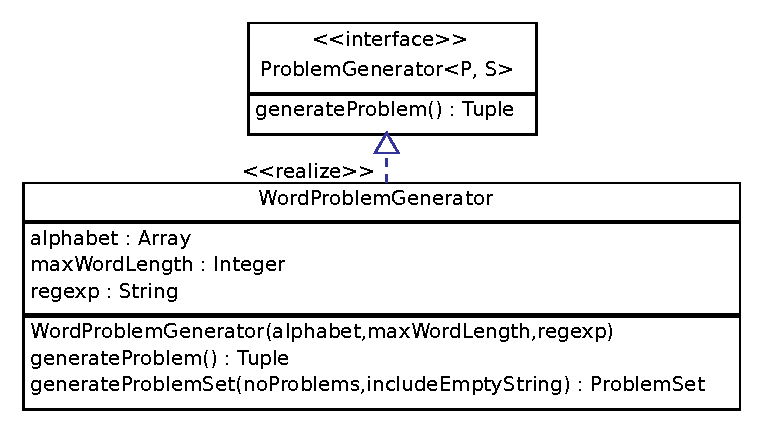
\includegraphics[width=0.5\textwidth]{images/simple_uml_pg.pdf}
  \caption[Problemgenerierung Klassendiagramm]{Problemgenerierung Klassendiagramm}
  \label{fig:ea_pg_classdiag_simple}
\end{figure}


\paragraph{Generieren von Lösungskandidaten}
Das Generieren von zufälligen Automaten mit einem gegebenen Alphabet erledigt der Konstruktor der \lstinline$RandomDeterministicFiniteAutomaton$ Klasse. Eine detaillierte Beschreibung wie die Automaten zufällig zusammengestellt werden befindet sich im Kapitel \ref{subsec:RandomDeterministicFiniteAutomaton}.

\subsubsection{Feste globale Problemmenge}
\subsubsection{Mutierende globale Problemmenge}
Die Implementation des Algorithmus mit der mutierenden globalen Problemmenge ist nahezu identisch mit der zuvor beschriebenen.

Sie unterscheidet sich lediglich darin, dass nach dem mutieren der Lösungskandidaten auch die Problemmenge verändert wird.

\begin{enumerate}
\item Initialisierung (Sprache, Problemmenge, Lösungskandidaten, Referenzautomat)
\item Berechnen der Fitness aller Lösungskandidaten
\item Sortieren der Lösungskandidaten nach Fitness
\item Hat ein Lösungskandidat alle Probleme korrekt gelöst? Falls ja, wird er mit dem Referenzautomaten verglichen. Wenn er einer korrekten Lösung entspricht wird der Algorithmus angehalten und die Anzahl gebrauchter Zyklen wird zurückgegeben.
\item Von den besten 50\% der Lösungskandidaten wird eine \textit{Deep Copy} erstellt
\item Die kopien werden zufällig mutiert
\item Die besten 50\% und deren mutierte kopien bilden die neue Menge der Lösungskandidaten.
\item \textbf{Die 50\% einfachsten Probleme aus der Problemmenge werden gelöscht und durch zufällige, neue ersetzt.}
\item Die Variable zum zählen der Zyklen wird um 1 erhöht.
\item Wenn das Zykluslimit noch nicht überschritten ist, weiter mit 2. ansonsten war der Algorithmus nicht erfolgreich und bricht ab.
\end{enumerate}
\subsubsection{Lokale mutierende Problemengen}
\label{subsec:LocalEvolvingProblemSet}
Der evolutionäre Algorithmus mit den lokalen mutierenden Problemmengen basiert auf einem anderen Prinzip. Hier treten jeweils zwei Kandidaten gegeneinander an und versuchen die Mitgeführten Probleme des Gegenspielers zu lösen. Derjenige der besser abschneidet gewinnt und kommt eine Runde weiter.

\begin{enumerate}
\item Initialisierung (Sprache, Lösungskandidaten mit einer Problemmenge pro Kandidat, Referenzautomat)
\item Durchiterieren der Liste der Lösungskandidaten in Zweierschritten (\lstinline$i+=2$). Selektion des von \lstinline$i$ten und \lstinline$i+1$ten Lösungskandidaten
\item Berechnung der Fitness des \lstinline$i$ten Lösungskandidaten unter Verwendung des Problem Sets des \lstinline$i+1$ten Lösungskandidates
\item Berechnung der Fitness des \lstinline$i+1$-ten Lösungskandidaten unter Verwendung des Problem Sets des \lstinline$i$-ten Lösungskandidates
\item Hat einer Lösungskandidat alle Probleme korrekt gelöst? Falls ja, wird er mit dem Referenzautomaten verglichen. Wenn er einer korrekten Lösung entspricht wird der Algorithmus angehalten und die Anzahl gebrauchter Zyklen wird zurückgegeben
\item Ist die Fitness der beiden Lösungskandidaten gleich? Falls ja, wird zufällig einer selektiert. Falls nein, wird vom Lösungskandidaten mit der höheren Fitness selektiert
\item Vom selektierten Lösungskandidaten wird eine \textit{Deep Copy} erstellt und zufällig mutiert
\item Die 50\% einfachsten Probleme der Problemmengen vom selektierten Lösungskandidaten und der Kopie werden gelöscht und durch zufällige, neue ersetzt 
\item Der selektierte Lösungskandidat und die mutierte Kopie werden der Liste der Lösungskandidaten der nächsten Runde hinzugefügt
\item Die Liste der Lösungskandidaten der nächsten Runde wird durchmischt (Die Reihenfolge der Lösungskandidaten wird randomisiert)
\item Wenn das Zykluslimit noch nicht überschritten ist, weiter mit 2. ansonsten war der Algorithmus nicht erfolgreich und bricht ab
\end{enumerate}
\subsection{Messen und Auswerten}
Bei ersten Versuchsreihen hat sich gezeigt, dass die evolutionären Algorithmen nicht in jedem Falle in einer annehmbaren Zeit konvergieren. Abhängig von der Grösse der Population und der Grösse der Problemmenge und des betrachteten Problems wurden Unterschiede im Konvergenzverhalten festgestellt.

Zum Vergleichen der verschiedenen Algorithmen wurden verschiedene Werte für die Grössen der Problemmenge und der Population gewählt. Die Algorithmen werden mit diesen, wechselnden, Eingabeparametern laufen gelassen und es wird gemessen wie oft die Algorithmen in annehmbarer Zeit eine Lösung finden. Dieser Wert wird dann auf eine Zahl zwischen 0 und 100 herunter skaliert um vergleichbare Werte zu erhalten. Zum Schluss werden diese Werte visualisiert.

Dieser Ablauf wurde in zwei Schritte unterteilt. In einem ersten Schritt laufen Java-Konsolenanwendungen und versuchen gegebene Probleme mit verschiedenen Eingabeparametern zu lösen. Sie loggen diese Ergebnisse in Logfiles mit folgendem Format:

\begin{lstlisting}[caption={Log Format}, label={lst:log_format}]
Mon Dec 30 06:05:10 CET 2013: Problem Count: 150
Mon Dec 30 06:05:10 CET 2013: CandidatesCount: 250
Mon Dec 30 06:05:10 CET 2013: Max Cycles: 500
Mon Dec 30 06:05:20 CET 2013: 0: finished (9245ms, 500cycles)
Mon Dec 30 06:05:20 CET 2013: 0: No solution found.
...
Mon Dec 30 06:14:53 CET 2013: 76: finished (812ms, 43cycles)
Mon Dec 30 06:14:53 CET 2013: 76: Solution found.
...
Mon Dec 30 06:17:34 CET 2013: 99: finished (12438ms, 500cycles)
Mon Dec 30 06:17:34 CET 2013: 99: No solution found.
Mon Dec 30 06:17:34 CET 2013: Solution Found: 37
Mon Dec 30 06:17:34 CET 2013: Avg cycles: 71
Mon Dec 30 06:17:34 CET 2013: Max cycles: 261
Mon Dec 30 06:17:34 CET 2013: Min cycles: 14
Mon Dec 30 06:17:34 CET 2013: No solution found: 63
Mon Dec 30 06:17:34 CET 2013: logging finished. (runtime: 744178ms)
\end{lstlisting}

In diesem Beispiel wurde ein Algorithmus mit einer 250 Problemen, 150 Individuen und einem Zykluslimit von 500 laufen gelassen. In 37 von 100 Fällen wurde eine Lösung gefunden. Bei den erfolgreichen Versuchen wurde durchschnittlich nach 71 Zyklen die Lösung entdeckt. Im schnellsten Fall war die Lösung bereits nach 14 Zyklen gefunden, im langsamsten Fall dauerte die Lösungsfindung 261 Zyklen.

Die Java-Konsolenanwendungen sind im Package \lstinline$ch.zhaw.regularLanguages.evolution.runners$ implementiert.

Im zweiten Schritt werden diese Logfiles von einem Python Script ausgelesen, Logfiles mit dem selben Präfix und der selben Problem- und Populationsgrössen werden zusammengefasst. Am Schluss werden die Ergebnisse mithilfe der Python Matplotlib \cite{matplotlib} geplottet. Das Python Script ist unter \lstinline$doc/statistics/log_analysis.py$ hinterlegt.

Um Vergleichswerte zu haben, wurde ein Zufallsalgorithmus implementiert, welcher versucht die Probleme durch einfaches ausprobieren zufälliger Automaten zu lösen. Die Erfolgsquote dieses Algorithmus wurde in die selbe Form gebracht wie diejenige der anderen.
\section{Supi5}

\clearpage

%%%
%%% end main document
%%%
%%%%%%%%%%%%%%%%%%%%%%%%%%%%%%%%%%%%%%%%%%%%%%%%%%%%%%%%%%%%%%%%%%%%%%%%%%%%%%%%

 \appendix  %% include it, if something (bibliography, index, ...) follows below
\section*{Protokoll Kick-Off Meeting}
\textbf{Steht die Auftraggeberin bzw. der Auftraggeber hinter dieser Semesterarbeit?}\newline 
Ja

\textbf{Sind die fachliche Kompetenz und die Verfügbarkeit der Betreuungsperson sichergestellt}\newline 
Ja

\textbf{Sind die Urheberrechte und Publikationsrechte geklärt?}\newline 
Ja

\textbf{Bekommt die Studentin oder der Student die notwendige logistische und beratende Unterstützung durch die Auftraggeberin bzw. den Auftraggeber?}\newline 
Es exitistert kein externer Auftraggeber

\textbf{Entsprechen Thema und Aufgabenstellungen den Anforderungen an eine Semesterarbeit?}\newline 
Ja

\textbf{Ist die Arbeit thematisch klar abgegrenzt und terminlich entkoppelt von den Prozessen (des Unternehmens) der Auftraggeberin bzw. des Auftraggebers?}\newline 
Ja

\textbf{Ist eine Grobplanung vorhanden? Sind die nächsten Schritte klar formuliert (von der Studentin oder dem Studenten)?}\newline 
Nächste Schritte:\\
\begin{itemize}
	\item Implementation von endlichen Automaten in Java
	\item Implementation von Automaten-Mutationen in Java
	\item Implementation grafischen Darstellung von endlichen Automaten
	\item Implementation der evolutionären Algorithmen
	\item Testen der Konvergenzverhaltne der verschiedenen implementationen
\end{itemize}

Dazu parallel:\\
\begin{itemize}
	\item Dokumentieren des erarbeiteten Wissens / erstellen des technischen Berichts.
\end{itemize}

\textbf{Ist die Arbeit technisch und terminlich von der Studentin oder dem Studenten umsetzbar?}\newline 
Ja

%%% start a new page and display the list of figures
% \newpage
 \listoffigures

%%% start a new page and display the list of tables
% \newpage
 \listoftables


%%%%%%%%%%%%%%%%%%%%%%%%%%%%%%%%%%%%%%%%%%%%%%%%%%%%%%%%%%%%%%%%%%%%%%%%%%%%%%%%
%%%
%%% bibliography
%%%
%%% available styles: abbrv, acm, alpha, apalike, ieeetr, plain, siam, unsrt
%%%
 \bibliographystyle{plain}

%%% name of the bibliography file
 \bibliography{projekt.bib}

\end{document}
%%% }}}
%%% END OF FILE
%%%%%%%%%%%%%%%%%%%%%%%%%%%%%%%%%%%%%%%%%%%%%%%%%%%%%%%%%%%%%%%%%%%%%%%%%%%%%%%%
%% Local Variables:
%% mode: outline-minor
%% OPToutline-regexp: "%% .*"
%% OPTeval: (hide-body)
%% emerge-set-combine-versions-template: "%a\n%b\n"
%% End:
%% vim:foldmethod=marker
